% !TeX spellcheck = en_GB
\documentclass[10pt]{beamer}
\usetheme{CambridgeUS}
%\usetheme{Boadilla}
\definecolor{myred}{RGB}{163,0,0}
%\usecolortheme[named=blue]{structure}
\usecolortheme{dove}
\usefonttheme[]{professionalfonts}
\usepackage[english]{babel}
\usepackage{amsmath,amsfonts,amssymb}
\usepackage{xcolor}
\usepackage{bm}
\usepackage{gensymb}
\usepackage{verbatim} 
\usepackage{paratype}
\usepackage{mathpazo}
\usepackage{listings}
\lstset{language=Python}

\usepackage{tikz}
\usetikzlibrary{matrix}

\DeclareMathOperator*{\interior}{int}

% Number theorem environments
\setbeamertemplate{theorem}[ams style]
\setbeamertemplate{theorems}[numbered]

% Reset theorem-like environments so that each is numbered separately
\usepackage{etoolbox}
\undef{\definition}
\theoremstyle{definition}
\newtheorem{definition}{\translate{Definition}}
\newtheorem{Fact}{\translate{Fact}}

% Change colours for theorem-like environments
\definecolor{mygreen1}{RGB}{0,96,0}
\definecolor{mygreen2}{RGB}{229,239,229}
\setbeamercolor{block title}{fg=white,bg=mygreen1}
\setbeamercolor{block body}{fg=black,bg=mygreen2}



\alt<presentation>
{\lstset{%
  basicstyle=\footnotesize\ttfamily,
  commentstyle=\slshape\color{green!50!black},
  frame = single,  
  keywordstyle=\bfseries\color{blue!50!black},
  identifierstyle=\color{blue},
  stringstyle=\color{orange},
  %escapechar=\#,
  showstringspaces = false,
  showtabs = false,
  tabsize = 2,
  emphstyle=\color{red}}
}
{
  \lstset{%
    basicstyle=\ttfamily,
    keywordstyle=\bfseries,
    commentstyle=\itshape,
    escapechar=\#,
    showtabs = false,
	tabsize = 2,
    emphstyle=\bfseries\color{red}
  }
} 

\title{R401: Statistical and Mathematical Foundations}
\subtitle{Lecture 15: Nonlinear Programming and Concave Optimization}
\author{Andrey Vassilev}

\date{2016/2017} 

\begin{document}
\maketitle



\begin{frame}[fragile]
\frametitle{Lecture Contents}
\tableofcontents
\end{frame}

\section{Static optimization with inequality constraints}\label{sec:ineq}

\begin{frame}[fragile]
\frametitle{Basic formulation with inequality constraints}
We now look at a problem which is very similar to the case of optimization with equality constraints:

\begin{equation}
f(x_1,\ldots,x_n)\rightarrow \max 
\label{eq:obj}
\end{equation}
s.t.
\begin{equation}
\begin{array}{l l l}
g_1(x_1,\ldots,x_n) \leq b_1\\
g_2(x_1,\ldots,x_n) \leq b_2\\
\cdots \\
g_m(x_1,\ldots,x_n) \leq b_m\\
\end{array}.
\label{eq:constr}
\end{equation}
In vector notation:
\[ f(\mathbf{x}) \rightarrow \max \]
s.t. \[ \mathbf{g}(\mathbf{x})\leq \mathbf{b}. \]
\end{frame}

\begin{frame}[fragile]
\frametitle{Basic formulation with inequality constraints}
\begin{itemize}
\item A vector $ \mathbf{x} $ satisfying the constraints \eqref{eq:constr} is called \emph{admissible} or \emph{feasible}.\bigskip
\item In some alternative (but essentially equivalent) formulations the constraints take the form
$ g_i(x_1,\ldots,x_n)\leq 0 $ or $ g_i(x_1,\ldots,x_n)\geq 0 $ for $ i=1,\ldots,m $.\bigskip
\item The set of admissible vectors is called the \emph{admissible (feasible) set}.\bigskip
\item With inequality constraints the requirement $ m<n $ is not necessary. Intuitively, this is because an inequality constraint is much more forgiving: think of a line vs. a half-plane.\bigskip
\item We focus on maximization problems here. Notice that minimizing a function $ f(x) $ is equivalent to maximizing $ -f(x) $, so there is no loss of generality in our choice.
\end{itemize}
\end{frame}

\begin{frame}[fragile]
\frametitle{Basic formulation with inequality constraints}
\framesubtitle{The Lagrangian}
We again approach problem \eqref{eq:obj}-\eqref{eq:constr} by defining a \emph{Lagrangian}:

\[ \mathcal{L}(\mathbf{x}) = f(\mathbf{x}) - \lambda_1 (g_1(\mathbf{x})-b_1) - \cdots - \lambda_m (g_m(\mathbf{x})-b_m). \]\bigskip

The Lagrangian takes the familiar form from the case of equality constraints! \bigskip

The differences arise in the algorithm used to obtain candidates for optimality.
\end{frame}

\begin{frame}[fragile]
\frametitle{Solution recipe for the case of inequality constraints}
When trying to find solutions to \eqref{eq:obj}-\eqref{eq:constr}, the following procedure is often applied:

\begin{block}{Algorithm (Kuhn-Tucker conditions)}
\begin{enumerate}
\item Form the Lagrangian
\item Differentiate it w.r.t. the elements of $ \mathbf{x} $ and set the resulting derivatives equal to zero:
\begin{equation}
\dfrac{\partial \mathcal{L}}{\partial x_i} = \dfrac{\partial f(\mathbf{x})}{\partial x_i} - \sum_{j=1}^{m}\lambda_j \dfrac{\partial g_j(\mathbf{x})}{\partial x_i} = 0,~i=1,\ldots,n.
\label{eq:dLdX}
\end{equation}
\item Check the \emph{complementary slackness} conditions \begin{equation}
\lambda_j \geq 0 \text{ and } \lambda_j (g_j(\mathbf{x})-b_j) = 0,~j=1,\ldots,m.
\label{eq:ComplSlack}
\end{equation}
\item The points satisfying 2) and 3) above are the candidates for optimality
\end{enumerate}
\end{block}

Condition 3) above implies that \[ \lambda_j = 0 \text{ if } g_j(\mathbf{x})<b_j,~j=1,\ldots,m. \]
\end{frame}

\begin{frame}[fragile]
\frametitle{Comments on the Kuhn-Tucker conditions}
\begin{itemize}
\item The term \emph{complementary slackness} derives from the fact that according to \eqref{eq:ComplSlack} one of the conditions $ \lambda_j \geq 0 $ and $ g_j(x_1,\ldots,x_n) \leq b_j $ may be \emph{slack} (i.e. be a strict inequality), while the other must bind (i.e. be fulfilled as an equality). Thus, they \emph{complement} each other. \bigskip
\item Let $ \mathbf{x^*} $ be an admissible point. If it is true that $ g_j(\mathbf{x^*})=b_j $, the respective constraint is called \emph{active} or \emph{binding}. \bigskip
\item It is possible to have simultaneously $ \lambda_j = 0 $ and $ g_j(\mathbf{x^*})=b_j $ for some $ j $s. 
\end{itemize}
\end{frame}

\begin{frame}[fragile]
\frametitle{A simple illustration of the Kuhn-Tucker procedure}
\begin{example}
\[ \max_{x,y} f(x,y) = xy \]
s.t. \[ x^2+y^2 \leq 1. \]

The Lagrangian is
\[ \mathcal{L} = xy - \lambda (x^2+y^2-1). \]
\[ \dfrac{\partial \mathcal{L}}{\partial x} = y-2\lambda x=0 \quad \Rightarrow \quad y = 2\lambda x, \]
\[ \dfrac{\partial \mathcal{L}}{\partial y} = x-2\lambda y=0 \quad \Rightarrow \quad x = 2\lambda y. \]

The complementary slackness condition reads \[ \lambda (x^2+y^2-1)=0. \]
\label{ex:KTillustrated}
\end{example}
\end{frame}

\begin{frame}[fragile]
\frametitle{A simple illustration of the Kuhn-Tucker procedure}\addtocounter{theorem}{-1}
\begin{example}[cont.]
Assume $ \lambda = 0 $. Then the conditions $ \frac{\partial \mathcal{L}}{\partial x}=\frac{\partial \mathcal{L}}{\partial y}=0 $ imply $ x=y=0$, which provides one candidate.\bigskip

Assume $ \lambda \neq 0 $. We have $ x^2+y^2 = 1 $. Note that $ x=0 $ would imply $ y=0 $ and vice versa, which would violate the condition $ x^2+y^2 = 1 $. Thus, $ x,y \neq 0 $. Then we obtain \[ \dfrac{x}{y}=\dfrac{y}{x} \quad \Rightarrow \quad x^2 = y^2. \]\bigskip
\end{example}
\end{frame}

\begin{frame}[fragile]
\frametitle{A simple illustration of the Kuhn-Tucker procedure}\addtocounter{theorem}{-1}
\begin{example}[cont.]
The result $ x^2 = y^2 $, combined with $ x^2+y^2 = 1 $, yields four possibilities: \[ \begin{array}{l l l l l l r}
(x,y) & = & \left(\frac{1}{\sqrt{2}},\frac{1}{\sqrt{2}}\right) & \Rightarrow & \lambda &=& \frac{1}{2},\\
(x,y) & = & \left(-\frac{1}{\sqrt{2}},\frac{1}{\sqrt{2}}\right)& \Rightarrow &\lambda &=& -\frac{1}{2},\\
(x,y) & = & \left(\frac{1}{\sqrt{2}},-\frac{1}{\sqrt{2}}\right)& \Rightarrow &\lambda &=& -\frac{1}{2},\\
(x,y) & = & \left(-\frac{1}{\sqrt{2}},-\frac{1}{\sqrt{2}}\right)& \Rightarrow &\lambda &=& \frac{1}{2} .
\end{array} \]

The second and third case can be excluded, as they are associated with $ \lambda<0 $. Thus, we are left with the candidates $ x=y=\frac{1}{\sqrt{2}} $ and $ x=y=-\frac{1}{\sqrt{2}} $ in addition to the candidate $ x=y=0$ obtained above. Note, however, that the last point yields a smaller value of the objective function and can be excluded.
\end{example}
\end{frame}

\begin{frame}[fragile]
\frametitle{From the Kuhn-Tucker algorithm to necessary conditions}
While the Kuhn-Tucker algorithm in its present form provides us with candidates, we need to strengthen it further to obtain proper necessary conditions for optimality.\pause

\begin{Fact}[Kuhn-Tucker necessary conditions]
Let $ \mathbf{x^*}=(x_1^*,\ldots,x_n^*)' $ be a solution to \eqref{eq:obj}-\eqref{eq:constr}. Suppose that the functions $ f $ and $ g_i,~i=1,\ldots,m ,$ have continuous partial derivatives on a set $ S\subseteq \mathbb{R}^n $, and $ \mathbf{x^*} \in \interior S $. Suppose also that the gradients of the constraints which are binding at $ \mathbf{x^*} $, are linearly independent, i.e. if $ K := \{k~\vert~ g_k(\mathbf{x^*})=0\} $, it is true that \[ \nabla g_k(\mathbf{x^*}),~k\in K, \text{ are linearly independent.} \]

Then there exist unique numbers $ \lambda_1,\ldots,\lambda_m $ such that conditions \eqref{eq:dLdX} and \eqref{eq:ComplSlack} hold at $ \mathbf{x^*} $.
\label{fc:KT_NCs}
\end{Fact}\bigskip

The linear independence condition in Fact \ref{fc:KT_NCs} is called the \emph{constraint qualification (CQ)}.
\end{frame}

\begin{frame}[fragile]
\frametitle{An equivalent formulation of the constraint qualification}
Take the \emph{Jacobian} of the constraint function $ \mathbf{g}(\mathbf{x}) $ and remove the rows that correspond to the inactive constraints:
\[ 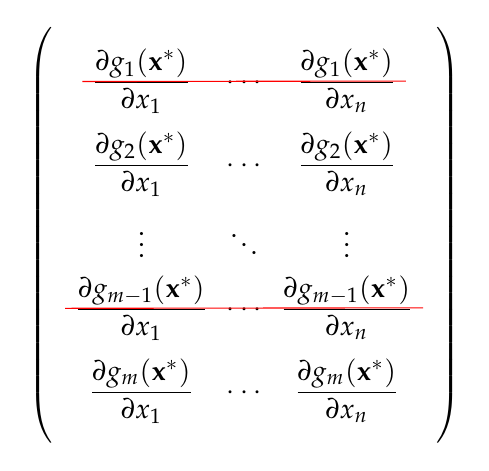
\begin{tikzpicture}
     \matrix (mat)[matrix of math nodes,left delimiter={(},right delimiter={)}]
      {%
		\dfrac{\partial g_1 (\mathbf{x^*})}{\partial x_1}  &  \cdots  &  \dfrac{\partial g_1 (\mathbf{x^*})}{\partial x_n} \\
		\dfrac{\partial g_2 (\mathbf{x^*})}{\partial x_1}  &  \cdots  &  \dfrac{\partial g_2 (\mathbf{x^*})}{\partial x_n} \\
		\vdots   &  \ddots  &  \vdots \\
		\dfrac{\partial g_{m-1} (\mathbf{x^*})}{\partial x_1}  &  \cdots  &  \dfrac{\partial g_{m-1} (\mathbf{x^*})}{\partial x_n} \\
		\dfrac{\partial g_{m} (\mathbf{x^*})}{\partial x_1}  &  \cdots  &  \dfrac{\partial g_{m} (\mathbf{x^*})}{\partial x_n} \\
      }; \pause
      \draw[red](mat-1-1.west) -- (mat-1-3.east);
      \draw[red](mat-4-1.west) -- (mat-4-3.east);
\end{tikzpicture}
\]

\uncover<3->{Here the first and the $ (m-1) $-th constraints are \textbf{not} binding.}
\end{frame}

\begin{frame}[fragile]
\frametitle{An equivalent formulation of the constraint qualification}
Thus, if $ k $ out of $ m $ constraints are not binding, we are left with a $ (m-k)\times n $ matrix of partial derivatives, evaluated at $ \mathbf{x^*} $.\bigskip

The constraint qualification requires that the rank of this matrix should be equal to the number of rows $ m-k $.
\end{frame}

\begin{frame}[fragile]
\frametitle{Applying the necessary conditions}
The CQ is a potential source of problems when applying the Kuhn-Tucker necessary conditions: it is possible to have an optimal point where the CQ (and hence the NCs) fail. \bigskip


Therefore the general procedure is as follows:
\begin{enumerate}
\item Use Fact \ref{fc:KT_NCs} to find a set of candidates.
\item Find the feasible points where the CQ fails. These are also candidates.
\item Search for the optimum over the union of the preceding two sets.
\end{enumerate}
\end{frame}

\begin{frame}[fragile]
\frametitle{Some illustrations}
\begin{example}
Consider the problem
\[ f(x_1,x_2) = -x_1^3+x_2 \rightarrow \max \]
s.t. \[ x_2\leq 0. \]

We have \[ \mathcal{L} =  -x_1^3+x_2 - \lambda x_2  \]
\[ \dfrac{\partial \mathcal{L}}{\partial x_1} = -3x_1^2 = 0 \quad \Rightarrow \quad x_1 = 0. \]
\[ \dfrac{\partial \mathcal{L}}{\partial x_2} = 1-\lambda = 0 \quad \Rightarrow \quad \lambda = 1. \]

Complementary slackness requires that $ \lambda x_2 = 0 $, hence $ x_2 = 0 $.
\label{ex:KTfail}
\end{example}
\end{frame}

\begin{frame}[fragile]
\frametitle{Some illustrations}\addtocounter{theorem}{-1}
\begin{example}[cont.]
The gradient of the constraint function is $\nabla g(x_1,x_2) = (g'_x(x_1,x_2),g'_y(x_1,x_2))' = (0,1)' $, so the CQ is satisfied everywhere. \bigskip

To sum up, the K-T NCs are satisfied and $ x_1=0,~x_2=0 $ is our only candidate.\bigskip

However, it is easily seen that any point of the type $ (x_1,0) $ with $ x_1<0 $ is admissible, and for $ x_1 \rightarrow -\infty $ the objective function grows unboundedly. 

This again illustrates the need to use NCs with caution. 
\end{example}
\end{frame}

\begin{frame}[fragile]
\frametitle{Some illustrations}
\begin{example}[Example \ref{ex:KTillustrated} revisited]
The solution of Example \ref{ex:KTillustrated} did not make use of the CQ condition. Let us check it now: \[ g(x,y)=x^2+y^2. \]
\label{ex:revisitKTillustrated}
\end{example}
\end{frame}


\section*{}
\begin{frame}[fragile]
\frametitle{Readings}
Main references:

Syds\ae{}ter et al. \emph{Further mathematics for economic analysis}. Chapter 3.\bigskip

Additional readings:
\end{frame}

\end{document}